\subsection{Experimentación}

\par Vamos a realizar diversos experimentos sobre las implementaciones de los dos algoritmos mencionados previamente (Top down y Bottom up) con el fin de comparar sus rendimientos y poder sacar conclusiones sobre ellos.

\par Algunos experimentos miden tiempos y comparan estos resultados con la cota de complejidad antes planteada. Por esto, vamos a definir algunos parámetros que nos van a servir para entendernos mejor:

\begin{itemize}
	\item \textit{$N$}: Cantidad de tipos de tesoros.
	\item \textit{$M$}: Cantidad de mochilas.
	\item \textit{$K_i$}: Capacidad de la mochila $i$.
	\item \textit{$C_i$}: Cantidad de tesoros del tipo $i$.
	\item \textit{$\sum_{i = 1}^{N} C_i$}: Cantidad total de tesoros. A partir de ahora nos referiremos a esta sumatoria como \textit{C}.
	\item \textit{$\sum_{i = 1}^{M} K_i$}: Capacidad total de todas las mochilas. A partir de ahora nos referiremos a esta sumatoria como \textit{K}.
\end{itemize}

\par La cota de complejidad planteada es O($(\sum_{i = 1}^{M} K_i)^{M} \cdot (\sum_{i = 1}^{N} C_i)$), que con la notación tomada nos queda O($K^{M} \cdot C$).

\subsubsection{Experimento 1: $\#$ Tesoros y Capacidad total de mochilas en aumento}

\par En el primer experimento, fijaremos la cantidad de mochilas (\textit{M}) y variaremos la cantidad total de tesoros (\textit{C}) y la capacidad total de mochilas (\textit{K}) para ver cómo se comportan y si cumplen la cota de complejidad antes mencionada.

\par Tomaremos M=1. Por lo tanto, la cota de complejidad nos queda O($K_1 \cdot C$). Vamos a ir aumentando los valores de $K_1$ y $C$ y tomaremos el tiempo que le toma al programa encontrar la solución y finalizar. Tanto la cantidad de tipos de tesoros, como los pesos y los valores de cada tipo de tesoro serán tomados al aleatoriamente en un rango entre 1 y $K_1$ (para que siempre pueda entrar en la mochila). Aumentaremos el valor $K_1$ mas rápidamente que $C$, para que al menos varios tesoros puedan entrar en la mochila (sabiendo que su peso está acotado por la capacidad de esta mochila).

\par Esperamos que, para ambas implementaciones, los tiempos se mantengan en un orden lineal con respecto a $K_i \cdot C$. Creemos que la implementación \textit{Bottom up} debe mantenerse con tiempos mayores con respecto a la implementación \textit{Top down}, ya que la primera va a calcular todas las casillas de la matriz, mientras que la segunda solo va a completar las necesarias.

\begin{figure}[H]
	\centering
	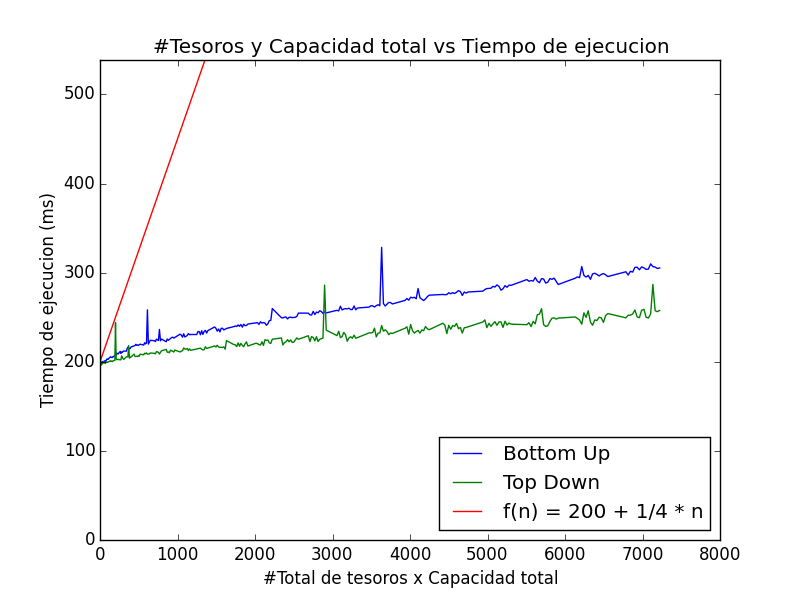
\includegraphics[width=0.9\textwidth]{Problema3/img/exp1_tiempos_general.png}
	\caption{Resultados del experimento 1.}
	\label{fig: exp1_tiempos_general}
\end{figure}

\par En la figura \ref{fig: exp1_tiempos_general} podemos ver los resultados del experimento. Sobre el eje x ubicamos el valor $K_1 \cdot C$ para poder observar si el gráfico de los tiempos obtenidos es de orden lineal. Notamos que en ambas implementaciones el orden efectivamente es lineal, aunque multiplicado por una constante muy baja. Podemos decir que las diferencias esperadas entre las implementaciones se cumplieron: \textit{Bottom up} se mantuvo siempre por encima de \textit{Top down}.

\subsubsection{Experimento 2: Tesoros con peso 1}

\par Para este experimento, vamos a partir del experimento 1 y le haremos ciertos cambios. Mantendremos fija la cantidad de mochilas (M = 1) y variaremos la cantidad de tesoros y la capacidad de la mochila. El cambio mas importante es que tomaremos siempre peso=1, para todos los tesoros. También tomaremos siempre $K_1 = C$.

\par Lo que queremos ver al tomar esta caracterización de la entrada, es un peor caso de la implementación \textit{Top down}. Esto se lo adjudicamos a que debe recorrer un porcentaje de la matriz mayor al del resto de los casos, ya que la cantidad de capacidades a las que puede llegar (como combinación de poner o no los objetos anteriores) es mayor. Veamos un ejemplo: nos ubicamos en la casilla M[i,j], donde \textit{i=número de tesoro} y \textit{j=capacidad disponible en la mochila}. Podemos agregar el tesoro a la mochila o no agregarlo. Como el tesoro tiene peso=1, debemos pasar a las casillas M[i+1,j] y a la M[i+1,j-1]. Podemos ver que no se saltean filas, porque los pesos son siempre 1. De esta forma se recorre un mayor porcentaje de casilleros. Si entramos en detalle se recorrerán exáctamente $\sum_{i=1}^{K_1}i = \frac{K_i \cdot (K_1 + 1)}{2}$ casilleros (no creemos que venga al caso la demostración, simplemente es un dato informativo).

\begin{figure}[H]
	\centering
	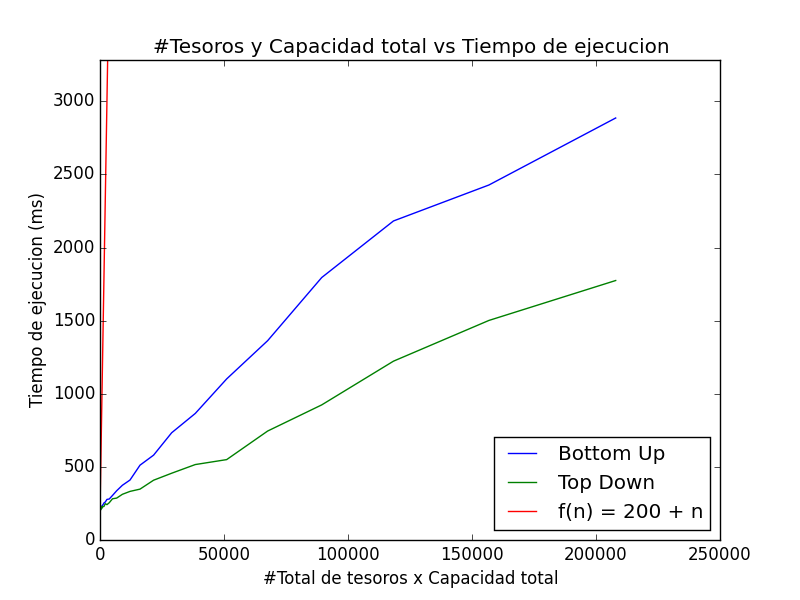
\includegraphics[width=0.9\textwidth]{Problema3/img/exp2_tiempos_peor.png}
	\caption{Resultados del experimento 2.}
	\label{fig: exp2_tiempos_peor}
\end{figure}

\par En la figura \ref{fig: exp2_tiempos_peor} podemos ver los resultados del experimento 2. Podemos ver que los tiempos de la implementación \textit{Top down} se mantienen por debajo de \textit{Bottom up}, a pesar de que creimos que este era un peor caso, y que podía influir en el rendimiento. Igualmente, los resultados se corresponden con lo esperado, ya que \textit{Bottom up} siempre recorre y calcula toda la matriz, mientras que habíamos mencionado que \textit{Top down} (en este caso) recorre $\frac{K_i \cdot (K_1 + 1)}{2}$ casilleros.

\par Antes de comparar los distintos casos para cada implementación veamos el siguiente experimento.

\subsubsection{Experimento 3: Tesoros muy pesados}

\par En el experimento 2 fijamos el peso en 1, haciendo que el algoritmo \textit{Top down} recorra gran parte de la matriz. En este experimento vamos a hacer lo contrario, fijaremos los pesos en un valor alto para que no pueda entrar en la mochila y se recorra muy poca parte de la matriz. Esto se lo adjudicamos al hecho de que al no poder colocar ningún tesoro en la mochila solo recorre una fila de la matriz. Veamos un ejemplo: nos ubicamos en la casilla M[i,j], donde \textit{i=número de tesoro} y \textit{j=capacidad disponible en la mochila}. No podemos agregar el tesoro a la mochila (por su peso), entonces solo podemos movernos a la casilla M[i+1,j]. De esta manera solo se recorre una fila: $C$ casillas.

\par Tomaremos una mochila (M=1), fijaremos el peso de cada tesoro en $K_i$+1 y veremos qué pasa con el rendimiento al ir aumentando $C$ y $K_1$.

\begin{figure}[H]
	\centering
	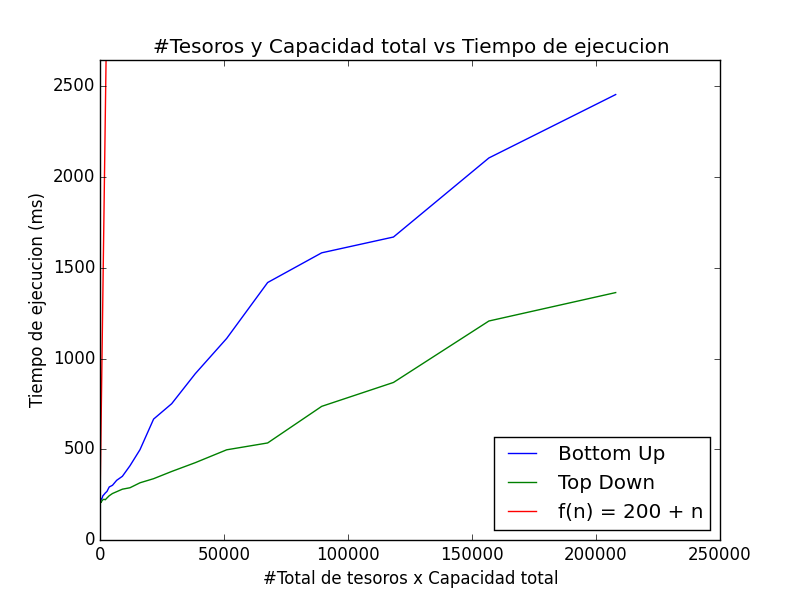
\includegraphics[width=0.9\textwidth]{Problema3/img/exp3_tiempos_mejor.png}
	\caption{Resultados del experimento 3.}
	\label{fig: exp3_tiempos_mejor}
\end{figure}

\par En la figura \ref{fig: exp3_tiempos_mejor} podemos ver los resultados del experimento. Notamos que los tiempos de la implementación \textit{Top down} son menores a los de los experimentos previos, pero no notamos una gran diferencia. Además, un dato interesante es que los tiempos de la implementación \textit{Bottom up} también disminuyeron. No sabemos concrétamente a qué se debe esto. Creemos que es porque al no entrar en algunas condiciones (por el excesivo peso de los tesoros) se evita algunas asignaciones y llamadas a funciones. Al tomarse tamaños de matriz tan grandes, tal vez este factor afecte levemente el rendimiento y esto sea lo que vemos reflejado en los resultados de los experimentos.

\par Ahora si, con estos últimos experimentos podemos comparar los resultados agrupándolos por implementación.

\begin{figure}[H]
	\centering
	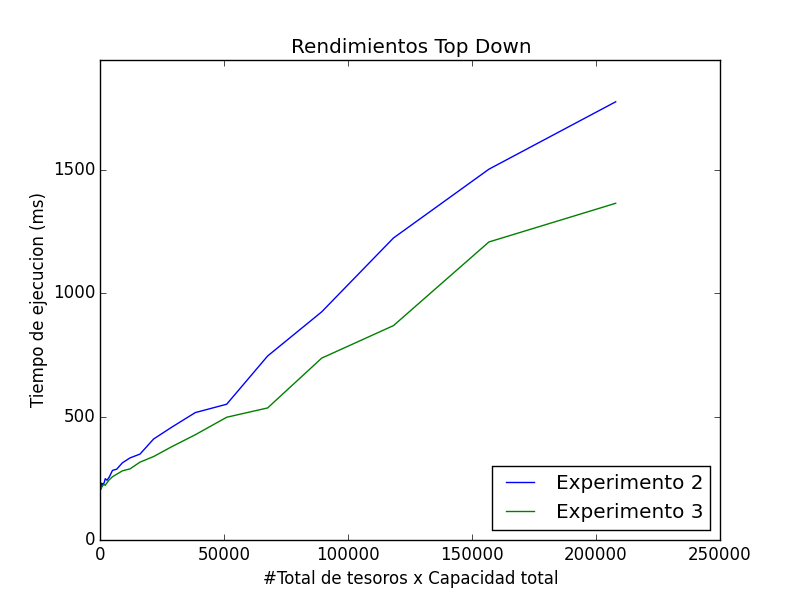
\includegraphics[width=0.9\textwidth]{Problema3/img/comparacion_td.png}
	\caption{Experimentos 2 y 3 - Top Down.}
	\label{fig: comparacion_td}
\end{figure}

\begin{figure}[H]
	\centering
	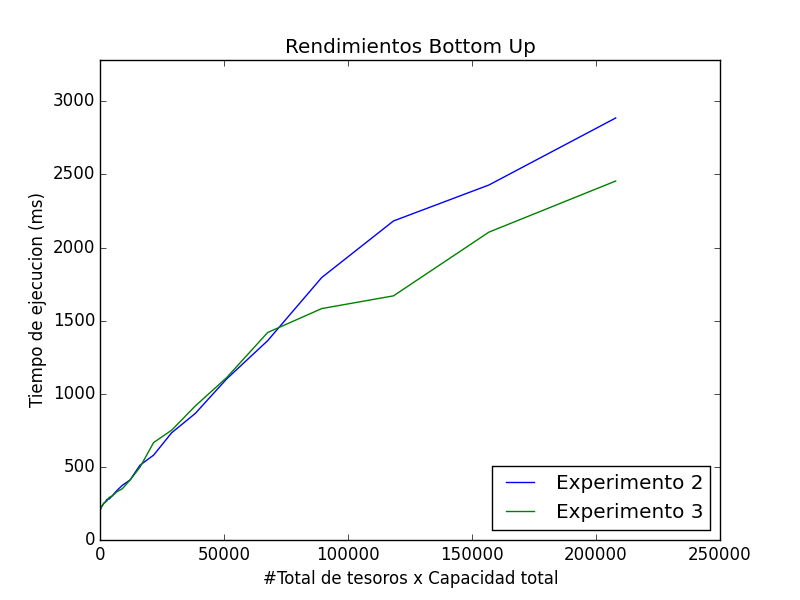
\includegraphics[width=0.9\textwidth]{Problema3/img/comparacion_bu.png}
	\caption{Experimentos 2 y 3 - Bottom Up.}
	\label{fig: comparacion_bu}
\end{figure}

\par En la figura \ref{fig: comparacion_td} podemos ver las diferencias entre el experimento 2 (nuestro peor caso) y el experimento 3 (nuestro mejor caso) en la implementación \textit{Top down}. Para el caso de la implementación \textit{Bottom up} se puede observar la figura \ref{fig: comparacion_bu}. Como mencionamos anteriormente, no creemos que esos casos sean mejores ni peores. Si creemos que hay factores que influyen levemente y se ven reflejados en el gráfico.

\subsubsection{Experimento 4: Medición de memoria}

\par Quedo claro que la implementación \textit{Top down} es mejor en cuanto a tiempos de ejecución que \textit{Bottom up}. Pero sabemos que la implementación \textit{Top down} se basa en una función que se llama recursivamente muchas veces hasta lograr calcular la solución al problema y creemos que esto puede impactar diréctamente sobre la memoria utilizada al momento de ejecutarse. Por lo tanto, en este experimento vamos a comparar la memoria utilizada por ambas implementaciones.

\par Vamos a enfocarnos en el peor caso de \textit{Top down} (experimento 2). La única diferencia será que no mediremos el tiempo de ejecución, sino la memoria utilizada. Para medir esta memoria utilizaremos funciones de java (\textit{Runtime}) que nos dan la memoria utilizada por el programa antes de ser administrada por el garbage collector.

\par Esperamos que en este caso, la mejor performance la tenga la implementación \textit{Bottom up}, ya que \textit{Top down} realiza muchas llamadas recursivas y acumulará muchos datos en el heap.

\begin{figure}[H]
	\centering
	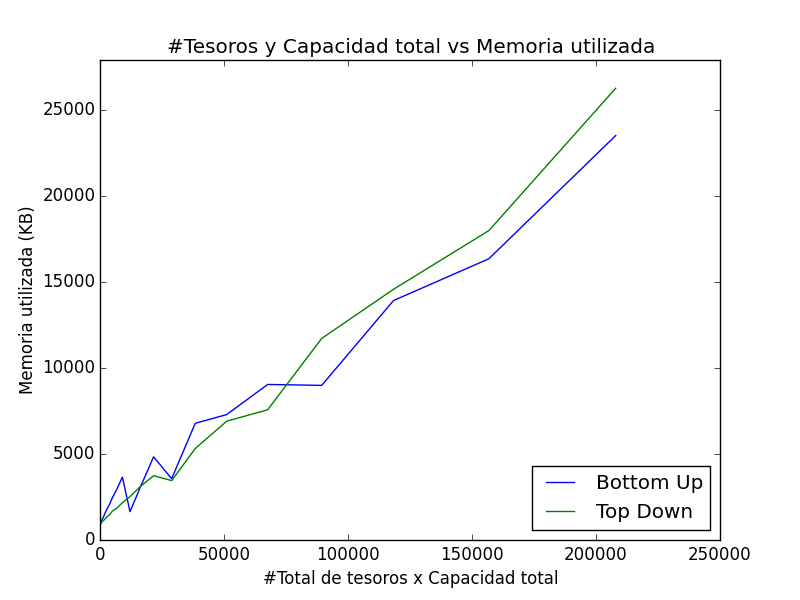
\includegraphics[width=0.9\textwidth]{Problema3/img/exp4_memoria.png}
	\caption{Resultados del experimento 4.}
	\label{fig: exp4_memoria}
\end{figure}

\par En la figura \ref{fig: exp4_memoria} podemos ver los resultados del experimento. Notamos que, a partir de un valor entre los 50000 y 100000, la implementación \textit{Top down} consume mas memoria que \textit{Bottom up}. Igualmente, esperábamos una diferencia mayor. No creemos que esta diferencia sea tan importante como para contrarestar los buenos resultados obtenidos en cuanto a tiempos de ejecución.

\smallskip

\par Luego de experimentar con las implementaciones, debemos decir que \textit{Top down} obtuvo una diferencia favorable en cuanto a tiempos y no se sobrepasó mucho en cuanto a memoria utilizada. Si debemos quedarnos con una implementación creemos que esta sería la elegida.